\documentclass[11pt,a4paper]{article}
\usepackage[utf8]{inputenc}
\usepackage[T1]{fontenc}
\usepackage[a4paper,top=1.9cm,bottom=2.2cm,left=2.3cm,right=2.3cm,headheight=14pt]{geometry}
\usepackage{amsmath,amssymb}
\usepackage{fancyhdr}
\usepackage{enumitem}
\usepackage{xcolor}
\usepackage[most]{tcolorbox}
\usepackage{tikz}
\usepackage{pgfplots}
\pgfplotsset{compat=1.18}

\pagestyle{fancy}
\fancyhf{}
\renewcommand{\headrulewidth}{0.4pt}
\renewcommand{\footrulewidth}{0.4pt}
\fancyfoot[L]{\textbf{Solucionario} -- simulacro de estudio}
\fancyfoot[R]{Página \thepage}
\setlength{\parindent}{0pt}
\setlength{\parskip}{1.5pt}

\definecolor{paso}{HTML}{252525}
\definecolor{res}{HTML}{8A29EB}
\definecolor{idea}{HTML}{B5651D}
\definecolor{ojo}{HTML}{D73E3E}
\newcommand{\sect}[1]{\vspace{8pt}{\large\bfseries #1}\par\vspace{-6pt}\rule{\linewidth}{0.4pt}\par}
\newcommand{\question}[2]{\vspace{6pt}\textbf{#1}\hfill\textbf{[#2]}\par}
\newcommand{\inciso}[1]{\vspace{4pt}{\bfseries\color{blue!60!black} #1}\par}
\newcommand{\paso}[1]{\tikz[baseline=-0.6ex]\node[circle,fill=paso,text=white,inner sep=1.2pt,font=\scriptsize\bfseries]{#1};\ }
\newcommand{\idea}[1]{{\color{idea}\textbf{Idea:}} #1\par}
\newcommand{\ojo}[1]{{\color{ojo}\textbf{Ojo:}} #1\par}
\newtcolorbox{resbox}{colback=res!6,colframe=res!70,boxrule=0.6pt,arc=2mm,left=4pt,right=4pt,top=2pt,bottom=2pt}
\newcommand{\res}[1]{\begin{resbox}\textbf{Resultado:} #1\end{resbox}}
\newcommand{\fbx}[1]{\boxed{\displaystyle #1}}

\begin{document}
\begin{center}
{\Large\bfseries ING340 Introducción a las Imágenes Médicas}\\[4pt]
{\large Solucionario del simulacro de parcial (paso a paso)}\\[2pt]
{\small\color{ojo} Solo para estudiar: tiene problemas resueltos, no lo lleves al examen.}
\end{center}

\sect{Ultrasonido}

% ================================================================ Q1
\question{Pregunta 1: Formación de haz con un arreglo lineal}{5.0 puntos}
\inciso{a) Lóbulos de rejilla}
\idea{prueba $m=\pm1$ en la fórmula de rejilla; si $|\sin\theta|>1$, ese lóbulo no existe.}
\paso{1} $\lambda = c/f_0 = 1540/(5\times10^{6}) = 0.308$ mm \quad;\quad $d/\lambda = 0.81$\par
\paso{2} Fórmula de la rejilla con steering:
\[ \fbx{\sin\theta_m = \sin\theta_s + \frac{m\lambda}{d}} \qquad\qquad \fbx{d < \frac{\lambda}{1+|\sin\theta_s|}} \]
\paso{3} Sin steering ($\theta_s=0$): $|\lambda/d| = 1.232 > 1$ $\Rightarrow$ \textbf{no hay} rejilla.\par
\paso{4} Con $\theta_s = 30^\circ$: $m=+1$: $0.5+1.232=1.732$ (no existe); $m=-1$: $0.5-1.232=-0.732$ $\Rightarrow$ $\theta=-47.1^\circ$.
\res{sí hay un lóbulo de rejilla en $\theta \approx -47.1^\circ$; para evitarlo se necesita $d < 0.308/1.5 = 0.205$ mm.}

\inciso{b) Nivel del lóbulo de rejilla}
\idea{el patrón total es elemento $\times$ factor de arreglo. El AF vale $N$ en el principal y en la rejilla; lo único que cambia es el factor del \textbf{elemento}, que NO se gira con el steering.}
\[ \fbx{H(\theta) = \underbrace{\mathrm{sinc}\!\left(\frac{w\sin\theta}{\lambda}\right)}_{\text{elemento}}\cdot AF(\theta)} \qquad \fbx{\Delta dB = 20\log\frac{E(\theta_{rej})}{E(\theta_s)}} \]
\paso{1} Principal: $w\sin30^\circ/\lambda = 0.22\cdot0.5/0.308 = 0.357$ $\Rightarrow$ sinc $=0.803$.\par
\paso{2} Rejilla: $w\,|\sin\theta|/\lambda = 0.22\cdot0.732/0.308 = 0.523$ $\Rightarrow$ sinc $=0.607$.
\res{$\Delta dB = 20\log(0.607/0.803) = -2.4$ dB: el lóbulo de rejilla es casi tan alto como el principal (genera ecos fantasma).}

\inciso{c) Ancho cero a cero con steering}
\[ \fbx{\sin\theta = \sin\theta_s \pm \frac{\lambda}{Nd}} \qquad \frac{\lambda}{Nd} = \frac{0.308}{32\cdot0.25} = 0.0385 \]
\res{$\theta = \arcsin(0.5385) = 32.58^\circ$ y $\arcsin(0.4615) = 27.48^\circ$ $\Rightarrow$ ancho $= 5.1^\circ$ (más ancho que sin steering).}

\inciso{d) Retardos de enfoque}
\idea{el elemento más LEJANO al foco dispara primero; la diferencia de retardos es la diferencia de distancias entre $c$.}
\paso{1} Foco: $x_f = r\sin30^\circ = 15$ mm, $z_f = r\cos30^\circ = 25.98$ mm.\par
\paso{2} Bordes del arreglo: $x = \pm(N-1)d/2 = \pm3.875$ mm.\par
\paso{3} Distancias:
\[ \fbx{r_n = \sqrt{(x_f-x_n)^2+z_f^2}} \]
\[ r_{izq}=\sqrt{18.875^2+25.98^2}=32.11\text{ mm},\qquad r_{der}=\sqrt{11.125^2+25.98^2}=28.26\text{ mm} \]
\paso{4} Diferencia de retardos y muestras:
\[ \fbx{\Delta\tau = \frac{r_{max}-r_{min}}{c}} = \frac{3.85\times10^{-3}}{1540} = 2.50\ \mu\text{s} \qquad \fbx{N_s = \Delta\tau\, f_s} = 2.50\times10^{-6}\cdot40\times10^{6} = 100 \]
\res{$\Delta\tau = 2.50\ \mu$s $=100$ muestras; dispara primero el elemento del borde \textbf{izquierdo} ($x=-3.875$ mm), el más lejano al foco.}

\inciso{e) Frame rate}
\paso{1} Líneas: $90^\circ/1^\circ + 1 = 91$; cada foco en Tx es otro disparo ($n_{focos}=2$).\par
\paso{2} Tiempo por disparo: $2z_{max}/c = 0.30/1540 = 194.8\ \mu$s.
\[ \fbx{T_{frame} = N_l\, n_{focos}\,\frac{2z_{max}}{c}} = 91\cdot2\cdot194.8\ \mu\text{s} = 35.5\text{ ms} \]
\res{$FR = 1/T_{frame} \approx 28$ imágenes por segundo.}

% ================================================================ Q2
\question{Pregunta 2: Reflexión y transmisión}{4.0 puntos}
\inciso{a) Amplitudes de los 3 primeros ecos}
\paso{1} Velocidad del agua a $37^\circ$C y las impedancias $Z=\rho c$:
\[ c_w = 1400+4.5(37) = 1566.5\text{ m/s} \]
\[ Z_w = 1.5665,\qquad Z_g = 0.95\cdot1450 = 1.3775,\qquad Z_m = 1.07\cdot1580 = 1.6906\ \text{MRayl} \]
\paso{2} Coeficientes (de 1 hacia 2):
\[ \fbx{R_{12}=\frac{Z_2-Z_1}{Z_2+Z_1}} \qquad \fbx{T_{12}=\frac{2Z_2}{Z_1+Z_2}} \]
$R_{12}=-0.0642$,\; $T_{12}=0.9358$,\; $T_{21}=1.0642$,\; $R_{23}=+0.1021$,\; $R_{21}=+0.0642$.\par
\paso{3} Atenuación de ida y vuelta en la grasa:
\[ \fbx{p\acute{e}rdida_{dB} = 2\,\alpha_0\,f\,e} = 2\cdot0.6\cdot2\cdot1 = 2.4\text{ dB} \;\Rightarrow\; 10^{-2.4/20} = 0.759 \]
\paso{4} Amplitudes (T al bajar, R donde rebota, T al subir):
\[ \fbx{eco_1 = R_{12}} \qquad \fbx{eco_2 = T_{12}R_{23}T_{21}\cdot0.759} \qquad \fbx{eco_3 = T_{12}R_{23}R_{21}R_{23}T_{21}\cdot0.759^2} \]
\res{$eco_1 = -0.064$ (invertido), $eco_2 = +0.077$, $eco_3 = +3.8\times10^{-4}$ (rebote dentro de la grasa, casi invisible). El músculo es grueso: su cara inferior no da eco cercano, por eso el 3.\textsuperscript{er} eco es el rebote.}

\inciso{b) Dibujo: tiempos y duración}
\[ \fbx{t_1=\frac{2e_w}{c_w}} = \frac{0.04}{1566.5} = 25.5\ \mu\text{s} \qquad \fbx{\Delta t=\frac{2e_g}{c_g}} = \frac{0.02}{1450} = 13.8\ \mu\text{s} \qquad \fbx{\tau=\frac{N_c}{f_0}} = \frac{3}{2\times10^6} = 1.5\ \mu\text{s} \]
$t_2 = 39.3\ \mu$s,\; $t_3 = 53.1\ \mu$s. Como $\tau = 1.5\ \mu$s $\ll 13.8\ \mu$s, \textbf{no se solapan}.
\begin{center}
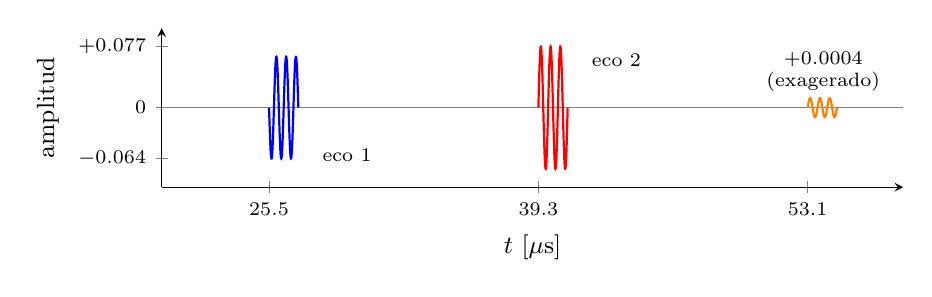
\begin{tikzpicture}
\begin{axis}[width=11cm,height=3.6cm,xmin=20,xmax=58,ymin=-0.1,ymax=0.1,axis lines=left,xlabel={$t$ [$\mu$s]},ylabel={amplitud},
 xtick={25.5,39.3,53.1},ytick={-0.064,0,0.077},yticklabels={$-0.064$,$0$,$+0.077$},yticklabel style={font=\scriptsize},xticklabel style={font=\scriptsize},samples=200,ylabel style={font=\small},xlabel style={font=\small}]
\addplot[gray,thin,domain=20:58] {0};
\addplot[blue,thick,domain=25.5:27.0] {-0.064*sin(deg(2*pi*2*(x-25.5)))};
\addplot[red,thick,domain=39.3:40.8] {0.077*sin(deg(2*pi*2*(x-39.3)))};
\addplot[orange,thick,domain=53.1:54.6] {0.012*sin(deg(2*pi*2*(x-53.1)))};
\node[font=\scriptsize] at (axis cs:29.5,-0.06) {eco 1};
\node[font=\scriptsize] at (axis cs:43.3,0.06) {eco 2};
\node[font=\scriptsize,align=center] at (axis cs:53.9,0.045) {$+0.0004$\\(exagerado)};
\end{axis}
\end{tikzpicture}
\end{center}

\inciso{c) Agua a $20^\circ$C}
\paso{1} $c_w = 1400+4.5(20) = 1490$ m/s $\Rightarrow$ $Z_w = 1.49$ MRayl.\par
\paso{2} $R_{12} = (1.3775-1.49)/(1.3775+1.49) = -0.0392$.
\res{el 1.\textsuperscript{er} eco baja $\approx39\%$ ($|{-0.0392}|/|{-0.0642}| = 0.61$), sigue invertido y llega más tarde ($t_1 = 0.04/1490 = 26.8\ \mu$s). El eco 2 casi no cambia (0.077). Comentario: al enfriarse, el agua se hace más lenta, su $Z$ se acerca a la de la grasa y refleja menos.}

% ================================================================ Q3
\question{Pregunta 3: Patrón de radiación de ultrasonido}{3.0 puntos}
\inciso{a) Patrón}
\idea{la fuente es un rect convolucionado con dos deltas; en Fourier la convolución es producto.}
\[ \fbx{U_0 = \mathrm{rect}\frac{x}{a} * \left[\delta\!\left(x-\tfrac{s}{2}\right)+\delta\!\left(x+\tfrac{s}{2}\right)\right]} \]
\[ H = a\,\mathrm{sinc}(au)\cdot2\cos(\pi s u),\qquad u=\frac{\sin\theta}{\lambda} \]
\res{$H_N(\theta) = \mathrm{sinc}\!\left(\dfrac{a\sin\theta}{\lambda}\right)\cos\!\left(\dfrac{\pi s\sin\theta}{\lambda}\right)$ con $\lambda = 1500/1.5\times10^6 = 1$ mm.}

\inciso{b) Ancho cero a cero}
\[ \fbx{\cos:\ \sin\theta=\frac{\lambda}{2s}} = 0.1 \Rightarrow 5.74^\circ \qquad \fbx{\mathrm{sinc}:\ \sin\theta=\frac{\lambda}{a}} = 0.5 \Rightarrow 30^\circ \]
\res{el primer cero es el del coseno ($5.74^\circ$) $\Rightarrow$ ancho cero a cero $= 11.5^\circ$.}

\inciso{c) Ancho a $-3$ dB}
\idea{primero supón sinc $\approx 1$, luego corrige con la tabla (una vuelta basta).}
\paso{1} $\cos(\pi s u) = 0.707 \Rightarrow \pi s u = \pi/4 \Rightarrow u = 1/(4s) = 0.05$ mm$^{-1}$ $\Rightarrow$ $\theta \approx 2.87^\circ$.\par
\paso{2} Ahí $au = 0.1$ $\Rightarrow$ sinc$(0.10)=0.984$ $\Rightarrow$ necesitas $\cos(\pi s u) = 0.707/0.984 = 0.718$ $\Rightarrow$ $\pi s u = 0.769$ $\Rightarrow$ $u = 0.0490$.
\res{$\theta_{-3dB} = \arcsin(0.0490) = 2.81^\circ$ $\Rightarrow$ ancho a $-3$ dB $\approx 5.6^\circ$.}

\inciso{d) Nivel a $15^\circ$}
\paso{1} $u = \sin15^\circ/1\text{ mm} = 0.2588$ mm$^{-1}$; $au = 0.518$ $\Rightarrow$ sinc $\approx 0.614$ (tabla, entre 0.50 y 0.52).\par
\paso{2} $\pi s u = 4.066$ rad $\Rightarrow \cos = -0.603$.
\[ \fbx{dB = 20\log|H_N|} = 20\log(0.614\cdot0.603) = 20\log(0.370) = -8.6\text{ dB} \]
\res{$-8.6$ dB. Sí hay lóbulos casi tan altos como el principal: los máximos del coseno ($\sin\theta = m\lambda/s = 0.2 \Rightarrow 11.5^\circ$) tienen nivel sinc$(0.4)=0.757 \Rightarrow -2.4$ dB. Como $s>\lambda$, las dos fuentes se comportan como un arreglo de 2 elementos con ``pitch'' grande (lóbulos tipo rejilla), solo atenuados por el sinc del ancho $a$.}

% ================================================================ Q4
\question{Pregunta 4: La ecuación de onda}{3.0 puntos}
\inciso{a) Cumple la ecuación de onda}
\paso{1} $rp = A\,e^{j(\omega t-kr)}$ $\Rightarrow$ $\dfrac{\partial^2(rp)}{\partial r^2} = (-jk)^2\,rp = -k^2\,rp$ $\Rightarrow$ $\nabla^2 p = -k^2 p$.\par
\paso{2} $\dfrac{\partial^2 p}{\partial t^2} = (j\omega)^2 p = -\omega^2 p$.\par
\paso{3} Reemplaza en $\nabla^2 p = \dfrac{1}{c^2}\dfrac{\partial^2 p}{\partial t^2}$: \; $-k^2 p = -\dfrac{\omega^2}{c^2}p$.
\res{se cumple porque $k = \omega/c$.}

\inciso{b) $u$, $\xi$ y $Z_{sp}$}
\paso{1} Derivada: $\dfrac{\partial p}{\partial r} = -\left(jk+\dfrac{1}{r}\right)p$.\par
\paso{2} Ecuación de movimiento $\rho_0\,\partial u/\partial t = -\partial p/\partial r$ con $\partial/\partial t \to j\omega$:
\[ \fbx{u = \frac{p}{\rho_0 c}\left(1+\frac{1}{jkr}\right)} \qquad \fbx{\xi = \frac{u}{j\omega}} \qquad \fbx{Z_{sp}=\frac{p}{u}=\rho_0 c\,\frac{jkr}{1+jkr}} \]
\ojo{si la onda fuera \emph{entrante}, $e^{j(\omega t+kr)}$, cambia $k\to-k$: $Z_{sp} = \rho_0c\,jkr/(1-jkr)$.}

\inciso{c) Distancias}
\paso{1} $k = 2\pi f/c = 2\pi(1000)/343 = 18.32$ m$^{-1}$.\par
\paso{2} Módulo y fase:
\[ \frac{|Z_{sp}|}{\rho_0c}=\frac{kr}{\sqrt{1+k^2r^2}} \ge 0.9 \;\Rightarrow\; \fbx{kr \ge \frac{1-\varepsilon}{\sqrt{1-(1-\varepsilon)^2}}} = 2.06 \]
\[ \text{fase} = \arctan\frac{1}{kr} \le 10^\circ \;\Rightarrow\; \fbx{kr \ge \cot\varphi_{max}} = 5.67 \]
\res{$r \ge 2.06/18.32 = 0.113$ m (módulo) y $r \ge 5.67/18.32 = 0.31$ m (fase).}

\inciso{d) Intensidad, potencia y nivel}
\[ \fbx{P_{ef} = P_{ref}\,10^{SPL/20}} = 20\ \mu\text{Pa}\cdot10^{4} = 0.2\text{ Pa} \qquad \fbx{I=\frac{P_{ef}^2}{\rho_0 c}} = \frac{0.04}{1.21\cdot343} = 9.6\times10^{-5}\ \text{W/m}^2 \]
\res{$W = 4\pi r^2 I = 1.2$ mW; a 4 m: $80 - 20\log(4) = 68$ dB (la presión cae como $1/r$).}

\sect{Rayos X}

% ================================================================ Q5
\question{Pregunta 5: Radiografía de proyección con dos energías}{3.0 puntos}
\inciso{a) Espesores}
\idea{una ecuación por cada energía, con $L=\ln(I_0/I)$; sistema 2$\times$2.}
\paso{1} $L_{30} = \ln(1/0.0174) = 4.051$; \; $L_{60} = \ln(1/0.187) = 1.677$.\par
\paso{2} Sistema:
\[ \fbx{\mu_{b}x_b+\mu_{m}x_m = L} \;\Rightarrow\; \begin{cases} 1.5\,x_b + 0.36\,x_m = 4.051\\ 0.45\,x_b + 0.20\,x_m = 1.677\end{cases} \qquad det = 1.5(0.2)-0.36(0.45) = 0.138 \]
\paso{3} Regla de Cramer:
\[ \fbx{x_b = \frac{L_{30}\mu_{m,60}-\mu_{m,30}L_{60}}{det}} = \frac{0.810-0.604}{0.138} \qquad \fbx{x_m = \frac{\mu_{b,30}L_{60}-\mu_{b,60}L_{30}}{det}} = \frac{2.515-1.823}{0.138} \]
\res{$x_b \approx 1.5$ cm de hueso y $x_m \approx 5.0$ cm de músculo.}

\inciso{b) Contraste}
\[ \fbx{C = 1-e^{-(\mu_b-\mu_m)x_b}} \;\Rightarrow\; C_{30} = 1-e^{-(1.14)(1.5)} = 0.82 \qquad C_{60} = 1-e^{-(0.25)(1.5)} = 0.31 \]
\res{más contraste a 30 keV: a baja energía domina el efecto fotoeléctrico ($\propto Z^3/E^3$) y el hueso (Z alto) atenúa mucho más que el músculo. El precio: pasa muy poca radiación (1.7\% frente a 18.7\%), así que hace falta más mAs y el paciente recibe más dosis.}

\sect{Tomografía computarizada}

% ================================================================ Q6
\question{Pregunta 6: Proyecciones y retroproyección}{2.0 puntos}
\inciso{a) Proyección a $0^\circ$}
\idea{región dentro de otra: usa linealidad, $g = \mu_{out}L_{out} + (\mu_{in}-\mu_{out})L_{in}$.}
\[ \fbx{g = \mu_{out}L_{out} + (\mu_{in}-\mu_{out})L_{in}} \qquad L_{out}=2 \ (|p|\le1),\quad L_{in}=2\sqrt{0.25-p^2}\ (|p|\le0.5) \]
\res{$g(p)=0.4+0.6\sqrt{0.25-p^2}$ si $|p|\le0.5$; \; $g=0.4$ si $0.5<|p|\le1$; \; $g=0$ si $|p|>1$. \; Valores: $g(0)=0.7$, $g(\pm0.5)=0.4$, $g(\pm1)=0.4$ (luego cae a 0).}
\begin{center}
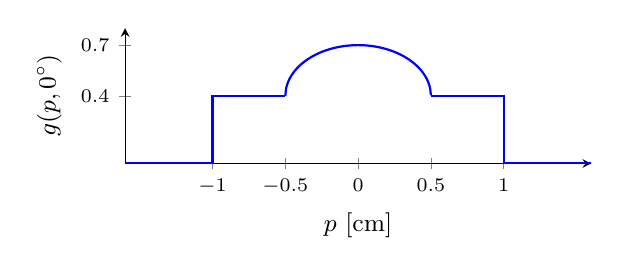
\begin{tikzpicture}
\begin{axis}[width=7.5cm,height=3.3cm,xmin=-1.6,xmax=1.6,ymin=0,ymax=0.8,axis lines=left,xlabel={$p$ [cm]},ylabel={$g(p,0^\circ)$},xtick={-1,-0.5,0,0.5,1},ytick={0.4,0.7},tick label style={font=\scriptsize},label style={font=\small},samples=200]
\addplot[blue,thick,domain=-1.6:-1] {0};
\addplot[blue,thick] coordinates {(-1,0) (-1,0.4) (-0.5,0.4)};
\addplot[blue,thick,domain=-0.5:0.5] {0.4+0.6*sqrt(max(0.25-x^2,0))};
\addplot[blue,thick] coordinates {(0.5,0.4) (1,0.4) (1,0)};
\addplot[blue,thick,domain=1:1.6] {0};
\end{axis}
\end{tikzpicture}
\end{center}

\inciso{b) $g(0,45^\circ)$}
\paso{1} El rayo por el centro a $45^\circ$ recorre la diagonal del cuadrado: $L_{out}=2\sqrt2=2.83$ cm; y el diámetro del círculo: $L_{in}=1$ cm.
\res{$g(0,45^\circ) = 0.2(2.83) + 0.3(1) = 0.87$.}

\inciso{c) Retroproyección en el origen}
\[ \fbx{\hat f(x,y) = g_0(x) + g_{90}(y)} \;\Rightarrow\; \hat f(0,0) = 0.7+0.7 = 1.4 \]
(si se pondera por $\Delta\theta$: $\times\,\pi/N = \pi/2 \Rightarrow 2.2$)\par
\res{1.4. Sale borrosa porque cada valor de la proyección se reparte a lo largo de TODO el rayo, también fuera del objeto (estrellas, borrosidad $\propto1/r$). La FBP primero filtra con la rampa $|q|$ y luego retroproyecta.}

\end{document}
